\section{嵌套虚拟化（一）：Turtles 与多层语义的单层复用}\label{sec:nested}


前两章分别考察了纯软件模拟与以 Arm 为代表的硬件辅助虚拟化，二者处理的都是“一层 hypervisor 直接管理一层 guest”的问题。本章把对象再推进一层：当 hypervisor 自己就跑在一台虚拟机里时，机器状态、地址映射与事件策略要如何组合才既正确又可接受地快。架构口径限定为 x86-64，即 amd64 这一 ISA 称谓，讨论的机制都落在 Intel 的 VMX 指令集、VMCS 控制结构与 EPT 扩展页表上，不使用 AMD SVM 的 VMCB/NPT 术语，也不把 Arm 的 EL2 异常级名称移植过来。嵌套这一问在文献里分成前后两段：OSDI 2010 年的 Turtles 回答“在缺乏架构支持时怎样正确实现嵌套”~\cite{source7}，USENIX ATC 2025 年的 HyperTurtle 回答“在已经能嵌套的前提下怎样减少不必要的跨层往返”~\cite{source8}。前一问是后一问的前提，二者不能按同一标准横向比较性能，只能按“谁控制资源、关键路径怎么走、何时介入、代价多大”这条主线先后展开。本章处理第一问，即多层语义如何被复用到底层的单层硬件支持上；下一章处理第二问，即往返成本如何削减。

\subsection{问题建立：当hypervisor自己也在虚拟机里}\label{sec:nested-problem}

嵌套虚拟化的层级用下标约定：L0 是跑在裸机上的 hypervisor，L1 是运行在 L0 虚拟机里的 guest hypervisor，L2 则是 L1 自己管理的嵌套 guest。L1 得到的机器接口必须包含它管理 L2 所需的虚拟化能力，即使真实 VMX 资源仍由 L0 控制；L2 则使用 L1 向它提供的虚拟机器接口~\cite{source7,source8}。

这一层次关系来自具体的部署需求。最直接的一类场景是租户自治：云厂商在 L0 上管理物理机，租户却希望在租给自己的虚拟机里再起 hypervisor，以便自行决定里面跑什么、如何迁移、何时快照，而无需惊动基础设施方。第二类是虚拟化软件自身的测试与开发——要复现“hypervisor 里再跑 hypervisor”的复杂环境，单层虚拟化天然不够。第三类，也是 HyperTurtle 论文最关心的，是基于虚拟机的安全容器：Kata 这类运行时用 microVM 而不是共享内核的进程来承载容器，换取更强的隔离边界；当这一层容器运行时本身又跑在租户的 VM（L1）里时，microVM 就成了 L2，嵌套就不再是可选项而是部署形态本身。必须澄清的是，并非所有容器都需要嵌套——普通容器共享宿主内核，不构成 L2；只有“在虚拟机内部再起 microVM”这一形态才触发本节讨论的问题，因此不能把容器隔离一律等同于嵌套虚拟化~\cite{source8}。

问题的难点不在“再多一层特权环”这样的直觉，而在资源归属的不对称。L1 确实要使用虚拟化扩展：它要执行 VMX 指令、创建自己的 VMCS、配置自己的 EPT。但真正的硬件资源——处理器当前运行所需的 VMX 状态、活动 EPT 上下文与真实 IOMMU——都由 L0 独占控制。于是 L0 面临的任务不是给 L1 一个更强的 ring，而是向 L1 提供一个“虚拟的虚拟化接口”：把 L1 要求的虚拟化操作接住、与 L0 自身对硬件和其余租户的约束合并，再组织成处理器当前可执行的一组硬件状态~\cite{source7}。

代价的直观体现是事件路径被拉长。当 L2 里发生一个需要 L1 处理的 VM-exit 时，CPU 先退出到 L0，L0 判断该事件需要向 L1 报告，并向 L1 反射退出，L1 处理完毕请求恢复 L2，L0 再次介入执行 VMEntry，最后才回到 L2，形成 $L2 \to L0 \to L1 \to L0 \to L2$ 的往返。但这条链不是所有事件都要走完：外部中断、NMI，以及只有 L0 在 VMCS02 里设置了 trap 而 L1 没在 VMCS12 里设置的事件，属于 L0 自己的范畴，L0 就地处理后直接恢复 L2，从 L1 的视角看这些事件根本不存在——正如单层虚拟化里 CPU 透明处理一次硬件事件后 hypervisor 继续运行一样~\cite{source7}。事件归属的判定权始终在 L0 手里，这才是“L0 保留最终控制”的准确含义，而不是“所有事件逐层转发”。

\subsection{Turtles：把多层语义组合到单层硬件支持上}\label{sec:turtles}

Turtles 是 KVM 之上的嵌套虚拟化实现，目标是运行未经修改的 guest hypervisor（KVM、VMware Server 等）及其 guest 系统。它在当时缺少专门嵌套硬件支持的条件下实现了可用的嵌套系统，并通过多类负载测量开销；论文的低开销结果不是对所有负载的统一上界。其实现涉及：CPU 上的 VMCS 合成、内存上的多维分页、I/O 上的多级设备分配，以及贯穿其中的退出归属判定~\cite{source7}。下面按四个维度分别说明“谁读写什么、怎样合成、代价在何处”。四维共同的骨架先由图~\ref{fig:turtles-arch} 固定。

\begin{figure}[htbp]
\centering
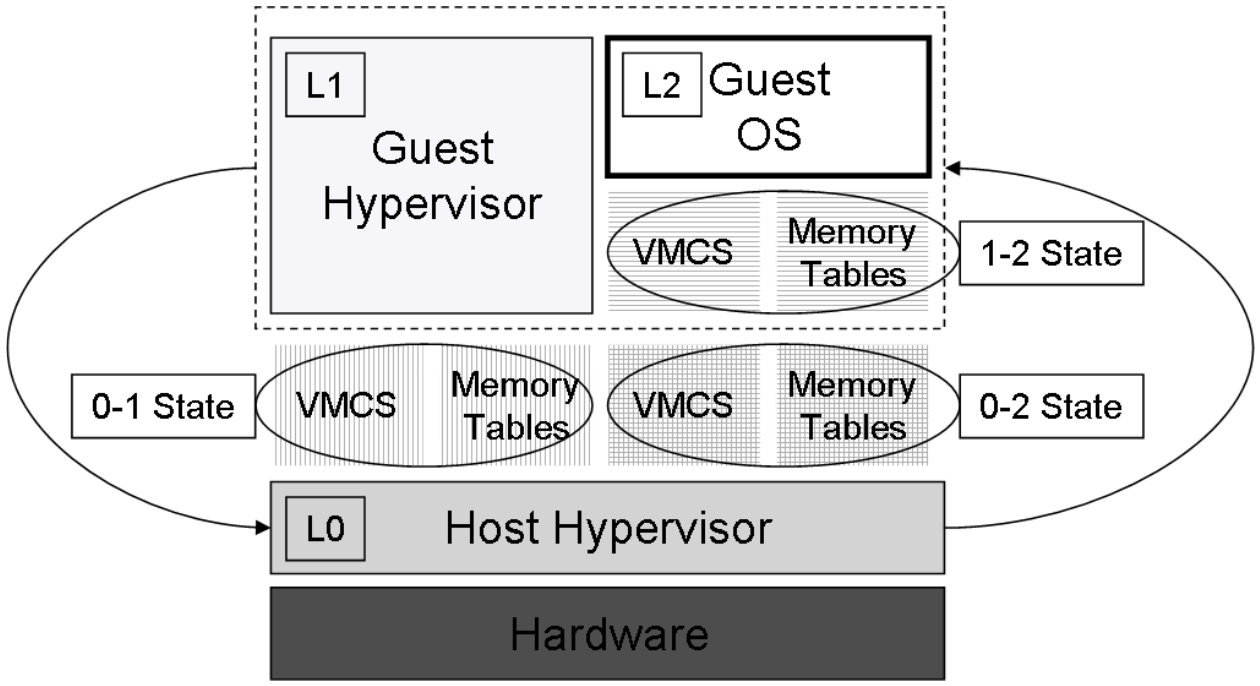
\includegraphics[width=0.82\linewidth]{figures/turtles-architecture.png}
\caption[嵌套虚拟化的总体架构]{嵌套虚拟化的总体架构：L1 与它管理的 L2 同处 L0 提供的一个虚拟机之内（虚线框），L0 为运行 L1 与运行 L2 各维护一份状态（0-1 与 0-2），L1 自己维护的 1-2 状态只存在于软件中。两侧弧形箭头表示 L0 与两台上层实体的运行关系：L0 借 0-1 状态运行 L1，借 0-2 状态运行 L2。引自 Ben-Yehuda et al., OSDI 2010, Figure 3~\cite{source7}。}
\label{fig:turtles-arch}
\end{figure}

图中三份状态都用 VMCS 与内存表（memory tables）两项表示，这正对应硬件虚拟化的两组对象：控制结构与地址翻译结构。0-1 是 L0 运行 L1 用的状态，0-2 是 L0 运行 L2 用的状态，二者都由 L0 维护并真正被硬件装载；1-2 是 L1 为 L2 准备的状态，图中以一个只存在于软件视角的方框表示——它从不进入处理器，只作为 L0 合成 0-2 的输入。同一张图也说明了嵌套的层级含义：硬件层之上只有 L0 一层 hypervisor 与它的虚拟机，L1 的“hypervisor 身份”完全由 L0 在软件中构造，这正是后面 CPU 与内存两节各自要展开的合成工作的出发点。

\subsubsection{CPU：虚拟化VMX与合成VMCS}\label{sec:nested-cpu}

在论文使用的单层 VMX 基线上，L1 在 VMX non-root 环境执行虚拟化管理指令会触发相应的拦截，这就给了 L0 一个天然的介入点：L0 捕获并模拟 L1 的 VMX 指令，也就是“trap-and-emulate”。大部分 VMX 指令的处理是“L1 退出到 L0、L0 按 VMCS 更新规则改写状态、再回到 L1”，让 L1 觉得指令真的执行了；但用来启动虚拟机的 \code{vmresume} 与 \code{vmlaunch} 是例外，因为此时 L0 必须模拟一次 L1→L2 的 VMEntry，流程变成“L1 退出到 L0，L0 直接 VMEntry 进入 L2”~\cite{source7}。

状态合成的关键是三份 VMCS 的分工，即图~\ref{fig:turtles-arch} 中三份状态各自的 VMCS 部分。VMCS01 是 L0 运行 L1 用的结构，从硬件角度看它和单层虚拟化完全一样：一个 hypervisor（L0）在 root mode 跑，一个 guest（L1）在 guest mode 跑。L1 为 L2 建立 VMCS12 来描述所需运行环境。该结构的地址与 host 状态具有 L1 视角下的含义，L0 不能不经检查、转换和合成就把它作为真实控制结构装载。于是 L0 以 VMCS12 为蓝本，再叠加 VMCS01 里对 L1 的约束，合成 VMCS02 作为真正运行 L2 的结构：guest state 大多可直接拷贝，host state 必须填成 L0 自己的、以便 CPU 从 L2 正确切回 L0，而 VMCS12 的 host state 要拷进 VMCS01 的 guest state，使 L0 模拟 L2→L1 切换时能加载正确的 L1 上下文~\cite{source7}。

控制数据的合成是正确性的重心。设想 L1 在 VMCS12 里要求 trap 某事件 $E_A$，但 L0 在 VMCS01 里并没有为 L1 trap 这个事件，那么为了把 $E_A$ 转发给 L1，L0 必须在 VMCS02 里补上对应的 trap；同理，L1 用来向 L2 注入事件的字段、以及 CPU 用来报告退出原因的字段都要合并。这套合并的具体实现落在 KVM 源码里，论文没有逐字段展开~\cite{source7}。这里有一个必须澄清的术语边界：Turtles 所说的 VMCS shadowing 是 L0 在软件层面“影子维护”VMCS12 并合成 VMCS02 的技术，与后来 Intel 在 Haswell 引入的同名硬件特性（让 L0 不必在每次 \code{vmread}/\code{vmwrite} 时都 trap）不是一回事；Turtles 的机制不依赖任何后续硬件能力~\cite{source7,source8}。同样，Turtles 描述的 2010 年合成逻辑，不应被当成当前 KVM 全部路径的写照——如今内核里的实现（如 \path{arch/x86/kvm/vmx/nested.c} 的 \code{prepare_vmcs02}）已经历多次重构并叠加了硬件加速，只可作为“合成 VMCS02 这一思路延续至今”的旁证，而非当年原型的源码~\cite{source5}。

\subsubsection{内存：EPT on top of EPT 的多维分页}\label{sec:nested-mem}

地址翻译在嵌套下多出一层：逻辑链是 L2 VA→L2 GPA→L1 GPA→host PA，即三层表。但当时的硬件 MMU 最多只支持两维（guest 页表 + EPT/NPT），无法同时走三层，因此必须把三层折叠到硬件提供的两层上。图~\ref{fig:turtles-mmu} 给出论文比较的三种折叠方式，区别在于哪一层由软件兜住：第一栏两层影子页表、第二栏影子页表叠在 EPT 上、第三栏才是 Turtles 采用的多维分页（图中标注为 EPT on top of EPT）。前两栏的共同点是 L1 用影子页表跑 L2，于是 L2 的每次页故障和每次页表写都要 L1 处理、并经 L0 转发；本节只展开第三栏，前两栏仅作为代价对照留在图上~\cite{source7}。

第三栏的关键是让两层都用 EPT 这一硬件结构，而不是让任何一层退化成影子页表。为此 L0 先向 L1 暴露 EPT 能力，使 L1 相信自己也能建 EPT，于是 L1 为 L2 建出 EPT12；但硬件只有一张 EPT，L0 不能直接装载 EPT12，便把它与自己的 EPT01 折叠成一张 EPT02。折叠的语义就是两次翻译的串接：L2 GPA 经 EPT12 得到 L1 GPA，再经 EPT01 得到 L0 的 host PA；EPT02 记录的是这条链的终点，因此硬件在实际执行时只需一次 EPT 遍历就完成 L2 GPA→host PA。图中第三栏下方那条从 L2 physical 直指 L0 physical 的 EPT02 箭头就是这个合成结果，而 EPT12 与 EPT01 两条箭头表示它由哪两段拼接而来；同时 L2 自己的页表（图中 GPT）仍然保留，负责 L2 VA→L2 GPA 这一层，硬件不替 L2 遍历它~\cite{source7}。

这张 EPT02 是按需建立的。L0 以一张空 EPT02 启动 L2，当 L2 访问的 GPA 在 EPT02 里缺项时触发 EPT violation 退出到 L0；L0 检查 L1 维护的 EPT12 是否已有该地址的合法映射——有，则把 EPT12 里的 L2→L1 映射与 EPT01 里的 L1→host 映射拼接后写入 EPT02 对应项；没有，说明这个缺页属于 L1 应负责的范围（例如 L1 尚未为该 GPA 分配内存），L0 就把退出交给 L1 处理，待 L1 更新 EPT12 后再回来补 EPT02~\cite{source7}。这个分流规则与 CPU 维度的退出归属判定同源：谁有权填这张表，缺项就归谁。

一致性维护是这套方案的固定开销。为保持 EPT02 与 EPT12 同步，L0 把 EPT12 所在内存设为只读，L1 一旦改写就 trap，L0 据此更新 EPT02 的相应项；L0 还要 trap L1 的 \code{INVEPT}，把 L1 意图的失效翻译成对自己 EPT 缓存的失效。两类 trap 的频率都由 EPT 表项数决定，因此 L0 允许用大页为 guest 内存做后备以缩小 EPT 表，也允许 L1 使用 VPID 给 TLB 条目打标签以免每次切换都冲刷 TLB；由于两侧都可自由选择 VPID 编号、可能冲突，L0 还需把 L1 自选的编号重映射到自己的有效编号~\cite{source7}。需要区分两类缺项：EPT02 缺项归 L0 补，L2 自身的普通页故障通常仍由 L2 处理，除非上层配置了相应拦截~\cite{source7}。

\begin{figure}[htbp]
\centering
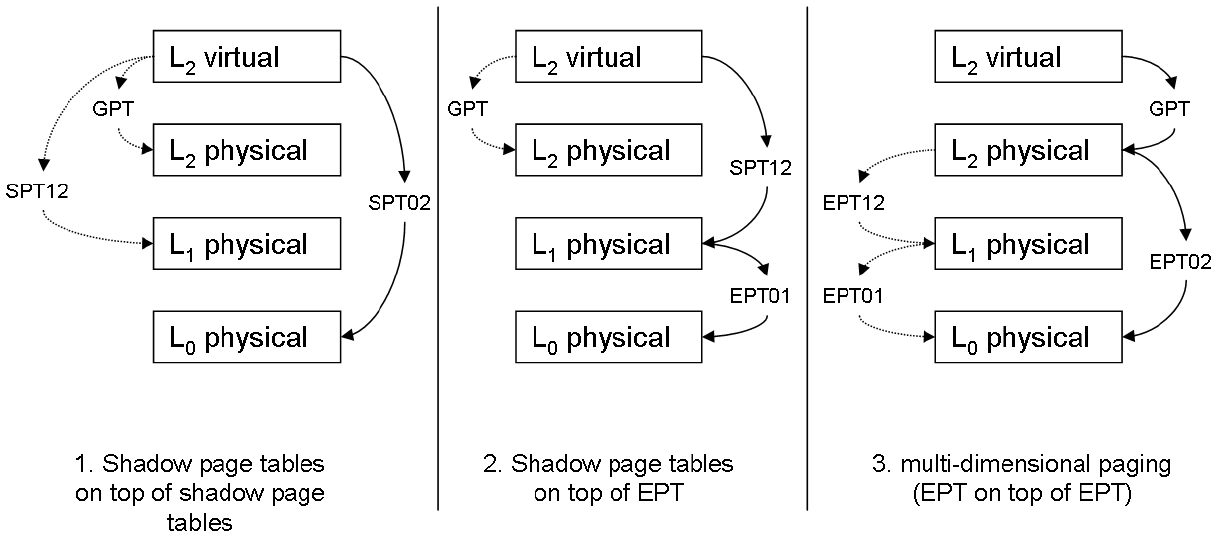
\includegraphics[width=0.98\linewidth]{figures/turtles-mmu-models.png}
\caption[三种嵌套 MMU 虚拟化模型]{三种嵌套 MMU 虚拟化模型：1. 影子页表叠在影子页表上；2. 影子页表叠在 EPT 上；3. 多维分页，即 EPT 叠在 EPT 上。四层方框自下而上为 L0 physical、L1 physical、L2 physical、L2 virtual，弧形箭头标注每段由哪张表承担（GPT、SPT12、SPT02、EPT01、EPT12、EPT02）。本文只展开第 3 栏。引自 Ben-Yehuda et al., OSDI 2010, Figure 4~\cite{source7}。}
\label{fig:turtles-mmu}
\end{figure}

\subsubsection{中断：事件归属、转发与注入}\label{sec:nested-irq}

嵌套下的中断必须分清三件不同的事：宿主自己产生的外部中断或 NMI，L0 要注入给 L1 的虚拟中断，以及 L1 希望注入给 L2 的事件。它们的处理路径不同。当 L2 正在运行且发生一次退出时，L0 首先按 VMCS12 与 VMCS02 的 trap 配置判断归属：属于 L0 的事件（外部中断、NMI，或只在 VMCS02 里 trap 的事件）就地处理后恢复 L2；属于 L1 的事件，L0 把 CPU 已更新的 VMCS02 字段拷回 VMCS12，再恢复 L1，让 L1 觉得是一次 L2→L1 的直接退出~\cite{source7}。注入方向上，L1 在 VMCS12 里写的注入字段要被 L0 合并进 VMCS02，才能让 CPU 真正把中断送进 L2。

设备分配场景揭示了一个关键的非对称性：DMA 直达不等于中断直达。多级设备分配让 L2 的数据可以直接落到设备，但中断在当时的 x86 架构上无法直接派发给 guest——中断到来总是先退出到 L0，L0 再转发 L1，L1 注入 L2，其中断的 EOI 写回也会再次触发退出。论文据此推断，设备中断及其 EOI 造成的退出是设备分配场景下残余开销的最大来源，并用一个去掉中断、纯轮询的网络驱动做了对照实验来支撑这一假设~\cite{source7}。需要强调的是，这是 2010 年原型在当时架构下的路径描述；后续硬件与 KVM 实现继续演进，因而不能把当年的中断处理路径断言为所有当前实现的必然行为~\cite{source7,source8}。

\subsubsection{设备：多级设备分配与虚拟IOMMU}\label{sec:nested-dev}

两层虚拟化各可选用模拟、半虚拟化或设备分配三种 I/O 方式，组合出九种可能，Turtles 重点评估了其中五种，并把“L0→L1 与 L1→L2 都做设备分配”称为多级设备分配~\cite{source7}。其目标不是把真实网卡“直通”给 L2 就完事，而是要在数据路径外补全三条辅助路径。

DMA 的地址问题是第一道坎：guest 驱动用的是 guest 物理地址，设备访存用的是 host 物理地址，而当时的 IOMMU 只支持一级翻译，两层映射必须再次压缩到一层。对可修改的 L1 可用半虚拟化 IOMMU——把 L1 里设置 L2→L1 映射的代码替换成对 L0 的 hypercall，L0 把映射里的 L1 地址换成对应 L0 地址后写入真实 IOMMU；对不改 L1 的方案，L0 为 L1 模拟一个 IOMMU，L1 以为自己在真 IOMMU 上建 L2→L1 映射，L0 截获这些映射、重映射 L1 地址、把 L2→host 的映射写到真实 IOMMU 上~\cite{source7}。中断路径如前所述仍需退出转发。MMIO 与 PIO 则相对干净：嵌套 guest 的 MMIO/PIO 与单层 guest 走同样的机制，不在 I/O 关键路径上引入额外退出~\cite{source7}。也就是说，多级设备分配的价值在于把 DMA 与 MMIO/PIO 留在直通路径上，代价集中在中断转发与 L1 注入这两类退出上，隔离和通知并没有被“直通”二字抹掉。

把四维放在一起看，Turtles 的“组合”有统一的形状：L1 表达的要求（VMCS12、EPT12、L1 侧的 IOMMU 映射）是输入，L0 自身的约束（VMCS01、EPT01、真实 IOMMU 的能力）是另一组输入，两者合并成一份硬件当下可执行的产物（VMCS02、EPT02、真实 IOMMU 里的映射表），而合并的依据始终是归属判定——退出归谁处理、缺项归谁填、设备地址归谁分配。图~\ref{fig:turtles-arch} 给出这一形状在整机层面的样子：三份状态中只有两份被硬件装载，第三份停留在软件里充当输入。

\subsection{Turtles 的开销与评测}\label{sec:turtles-cost}

Turtles 的成就是正确性与可行性：在不修改 guest hypervisor 的前提下给出了嵌套语义。但它的开销分析也暴露了问题的下一层形态。论文用 L2 里循环执行 \code{cpuid} 的合成微基准测单次退出的周期成本：裸机上 \code{cpuid} 约 100 周期，单层虚拟化约 2600 周期（其中约 1000 周期是模式切换），嵌套则飙到约 58000 周期~\cite{source7}。原因是 L1 每处理一次 L2 退出，都要执行多条 \code{vmread}/\code{vmwrite} 这类特权指令，而每条又各自触发一次对 L0 的退出——退出被逐级放大。论文在这里区分两类优化。L0 的合并路径可以只拷贝变化字段，并探索直接批量访问真实 VMCS 的方式；后一尝试不严格符合 VMX 规范，不能保证跨处理器适用。另一个称为 DRW 的评测配置则明确修改 L1，使其直接读写 VMCS12，用来估计省去 L1 的 VMREAD/VMWRITE 拦截的潜在收益。这两类直接访问不能混称为只修改 L0 的同一个优化~\cite{source7}。

论文的宏观负载报告给出同一方向的证据：在 KVM 同时充当 L0 与 L1 并启用多维分页的配置下，相对单层 guest，kernbench 的运行时间增加 14.5\%，SPECjbb 分数下降约 7.8\%；改用修改 L1、使其直接读写 VMCS12 的 DRW 配置后，两项数值分别变为 10.3\% 与 6.3\%~\cite[\S4.1, Table 2]{source7}。这些是论文报告值，不是本文复现。数值差异说明管理路径的密集程度会影响嵌套成本，摘要中的较低开销不能解释为适用于全部工作负载的上界；DRW 改动了 guest hypervisor，必须与未修改 guest 的基线分别讨论。

\subsection{小结：正确性之后剩下的成本}\label{sec:turtles-summary}

至此可以把 Turtles 的结论压成两句。正确性一侧，它把三层语义压进单层硬件支持：VMX 指令被 trap-and-emulate，VMCS12 作为需求说明书由 L0 合成为 VMCS02，EPT12 与 EPT01 折叠成 EPT02，L2 的 DMA 经虚拟或半虚拟 IOMMU 落到真实 IOMMU，而每一次退出由 L0 判定归属——属于它的事件就地处理后直接恢复 L2，属于 L1 的事件才转发。代价一侧，任何需要 L1 处理的退出都要走 $L2 \to L0 \to L1 \to L0 \to L2$，而 L1 处理时执行的 \code{vmread}/\code{vmwrite} 各自又触发一次对 L0 的退出，退出被逐级放大。两个边界需要重申：本章描述的是 2010 年原型在缺少嵌套架构支持时的实现，不能当作当前 KVM 全部路径的写照；DRW 这类配置改动了 guest hypervisor，其数字不能与未修改 guest 的结果混用。硬件后来加入的 VMCS shadowing 一类辅助改变的是复用的成本，而不是复用的必要性。成本究竟落在哪一段路径上、又该如何削减，是下一章的问题。
